\PassOptionsToPackage{unicode}{hyperref}
\PassOptionsToPackage{hyphens}{url}
%
\documentclass[superscriptaddress, 12pt]{revtex4-2}%twocolumn
\usepackage{amsmath,amssymb}
\usepackage{iftex}
% Use upquote if available, for straight quotes in verbatim environments
\usepackage{xcolor}
\usepackage{subcaption}
%\usepackage{longtable}
\usepackage{booktabs,array}
\usepackage{multirow}
\usepackage{calc} % for calculating minipage widths
% Correct order of tables after \paragraph or \subparagraph
\usepackage{etoolbox}
\usepackage{footnote}
\usepackage{graphicx}
\usepackage{bookmark}
%\usepackage{babel}
\IfFileExists{xurl.sty}{\usepackage{xurl}}{} % add URL line breaks if available
\urlstyle{same}
\hypersetup{
  hidelinks,
  pdfcreator={LaTeX via pandoc}}
\usepackage{textgreek}
\usepackage{makecell}
\usepackage{multirow}
\usepackage{booktabs}
\usepackage[LGR,T1]{fontenc}
\usepackage[utf8x]{inputenc}
\usepackage{textalpha}
\usepackage{ulem}
\usepackage{textcomp}
\usepackage{float}
\date{}


\newcommand{\MFnew}[1]{{\color{purple} #1}}
\newcommand{\MFmarginpar}[3]{\MFnew{#1} \marginpar{#2 \tiny \MFnew{#1 #3}}}

\begin{document}

\title{Influence of partial occupancy on the elastic tensor for FeCr \textsigma - phase.}

\author{Mariano Forti} \email{mariano.forti@icams.rub.de}
\affiliation{Interdisciplinary centre for advanced materials simulations (ICAMS), Ruhr Universität Bochum, Germany}

\author{Guillaume Laplanche} \email{}
\affiliation{Ruhr Universität Bochum}

\author{Thomas Hammerschmidt} \email{}
\affiliation{Interdisciplinary cetre for advanced materials simulations (ICAMS), Ruhr Universität Bochum, Germany}

\date{\today}

\maketitle

\section{Introduction}

The Fe-Cr system is an important alloy system with applications in structural and high-temperature environments.
The \textsigma-phase can form at Cr concentrations between 45 and 50\%at and temperatures ranging from 550 to 800\textdegree ~\cite{laplanche_phase_2018} significantly influencing the mechanical properties.
Specifically, \textsigma-phase precipitation contributes to embrittlement and reduces corrosion resistance {\color{red}  [ref 2 detrimental sigma] }.
The \textsigma-phase unit cell is shown in \autoref{fig:sigmaUnitCell}.
This is an intermetallic compound with a tetragonal structure (space group P4\textsubscript{2}/mnm) and exhibits complex atomic arrangements due to site-specific partial occupancies.
Understanding its properties is essential for predicting its mechanical behavior and phase stability.
There are different approaches to similar problems in atomistic simulations, based for instance on Density Functional Theory (DFT).
Vesti et. al. ~\cite{vesti_ab-initio_2023} utilize a full sublattice model later averaged under an ideal mixing approximation to interpolate the properties of a W-Re \textsigma phase.
Kabliman et. al. ~\cite{kabliman_ab_2012} use a mean field approximation to study several properties of the \textsigma phase in other binary systems, also based on full occupancy of the sublattices.
This assumption may overlook local atomic configuration effects.
In this work, we investigate how explicit consideration of partial occupancy influences the elastic properties of the \textsigma-phase through first-principles calculations.
We focus on a Fe16Cr14 unit cell which can be modelled with nominal and on-site compositions in agreement with experimental observations.

\begin{figure}
  \subcaptionbox{\protect\label{fig:sigmaUnitCell}}{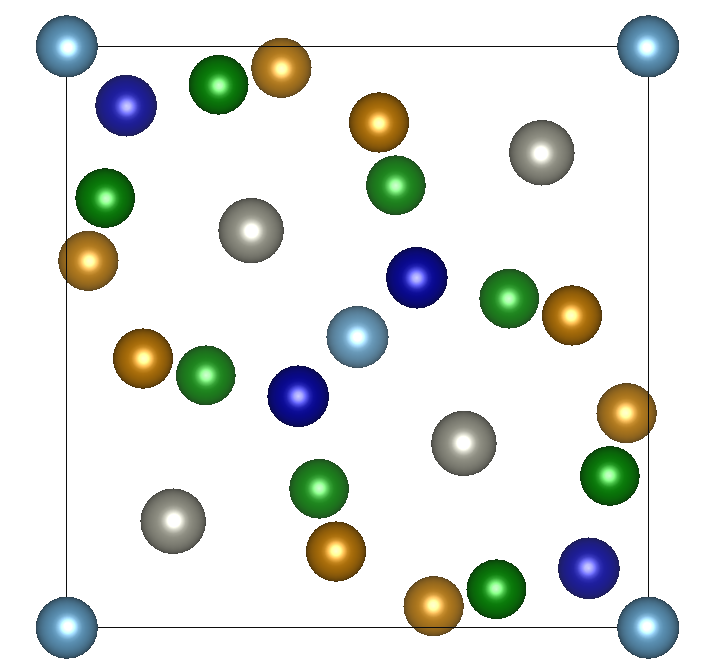
\includegraphics[height=4cm]{Figure_SigmaPhase001.png}}
  \caption{\protect\label{fig:introduction}
    (\subref{fig:sigmaUnitCell}) (001) view of the σ phase unit cell.
    Wyckoff sites are encoded in colors: 2a is light blue,
    4f in grey, 8i in green, 8i' in gold, 8j in blue.
  }
\end{figure}

\section{Methodology}

We employ first-principles DFT calculations to determine the elastic constants of the Fe-Cr \textsigma-phase. 
First, we study the change of elastic constansts with composition under a full site occupancy approximation.
Then, we focus on a nominal composition of Fe\textsubscript{16}Cr\textsubscript{14} (48\%at. Cr) to study the effect of partial occupancy explicitly.
These calculations are conducted using the Vienna Ab initio Simulation Package (VASP) ~\cite{Hafner_vasp}, utilizing the Perdew-Burke-Ernzerhof (PBE) ~\cite{Perdew1996} exchange-correlation functional and the Projector Augmented Wave (PAW) method ~\cite{Bloch1994, kresse_ultrasoft_1999}.
The elastic tensor is derived from stress-strain relationships obtained via energy-strain calculations~\cite{golesorkhtabar_elastic_2013}.

\paragraph{Full occupancy}

First, we calculate the properties of the \textsigma-phase using a full sublattice model.
This means, that the lattice positions of a WS are occupied either by Cr or Fe.
We calculate formation enthalpies and elastic constants for all the possible configurations spanning the full composition range.

\paragraph{Partial occupancy} To capture the impact of atomic disorder, we explicitly explore all possible atomic arrangements within the \textsigma~phase unit cell, incorporating experimentally reported partial occupancy of WS by Yakel~\cite{yakel_atom_1983} as reproduced in \autoref{fig:PartialOccupancies}.  
A random distribution in the different sublattices could be modelled for instance by a special quasirandom structure [SQS ref] but  this would require a big unit cell to generate a meaningful representation of such atomic distributions. 
In addition to this, the measured composition of the 2a site (< 0.5 atom per unit cell) would require an even bigger unit cell to model it accurately.
In order to keep the size of the simulation cell to one unit cell, we consider two approximations to the partial occupancy, in both cases disregarding Cr occupation in site 2a and rounding occupancy to integer numbers.  
A first model keeps one Fe atom in the site 4\textit{f} and 1 Cr atom in site 8\textit{i'}.  
In this condition, the total number of possible configurations is $ 1 \times 4 \times \binom{8}{3}\times \binom{8}{1} \times \binom{8}{3} \approx 100k $. 
We name this model 2\_A3B\_A5B3\_AB7\_A5B3.
A second model keeps the same number of atoms in the 8\textit{i} and 8\textit{j} sites, while transferring the Cr atom from 8\textit{i'} to 4\textit{f}.  
We call this other model B2\_A3B2\_A5B3\_B8\_A5B3. 
This reduces the number of possible configurations to $1 \times 1 \times \binom{8}{3}\times 1\times\binom {8}{3} = 3136$.~
In both models, the combinatorial explotion of the number of configurations hinders any extensive estimation of the elastic constants of a significant number of samples from DFT calculations, although in the second model the number of configurations is significantly reduced and approaching statistical significance would be easier.

Here we propose a combined DFT / machine learning interatomic potential (MLIP) approach to reduce the combinatorial sampling to the most relevant configurations, i.e. those with the lowest formation enthalpy.
As a first step, we select a subbset of 25 representative configurations of each model and calculate their optimized unit cell and their elastic constants using DFT. 
A specialized DFT dataset is built whcih consists of 
\begin{itemize}
	\item the relaxation path of all the full-occupancy samples,
	\item the relaxation paths of the 50 ad-hoc chosen partial-occupancy samples,
	\item random deformations including isotropic compresion and expansions and atom-position shaking, 
	\item relaxation paths for unit cell the optimization of the bcc, fcc, and hcp unary unit cells of the constitutents (Fe and Cr), 
	\item nearest neighbour expansions of the bcc, fcc, and hcp unary unit cells of the constituten elements (Fe and Cr)
\end{itemize}


\begin{figure}[h]
  
%  \subcaptionbox{\protect\label{fig:PartialOccupanciesA}}{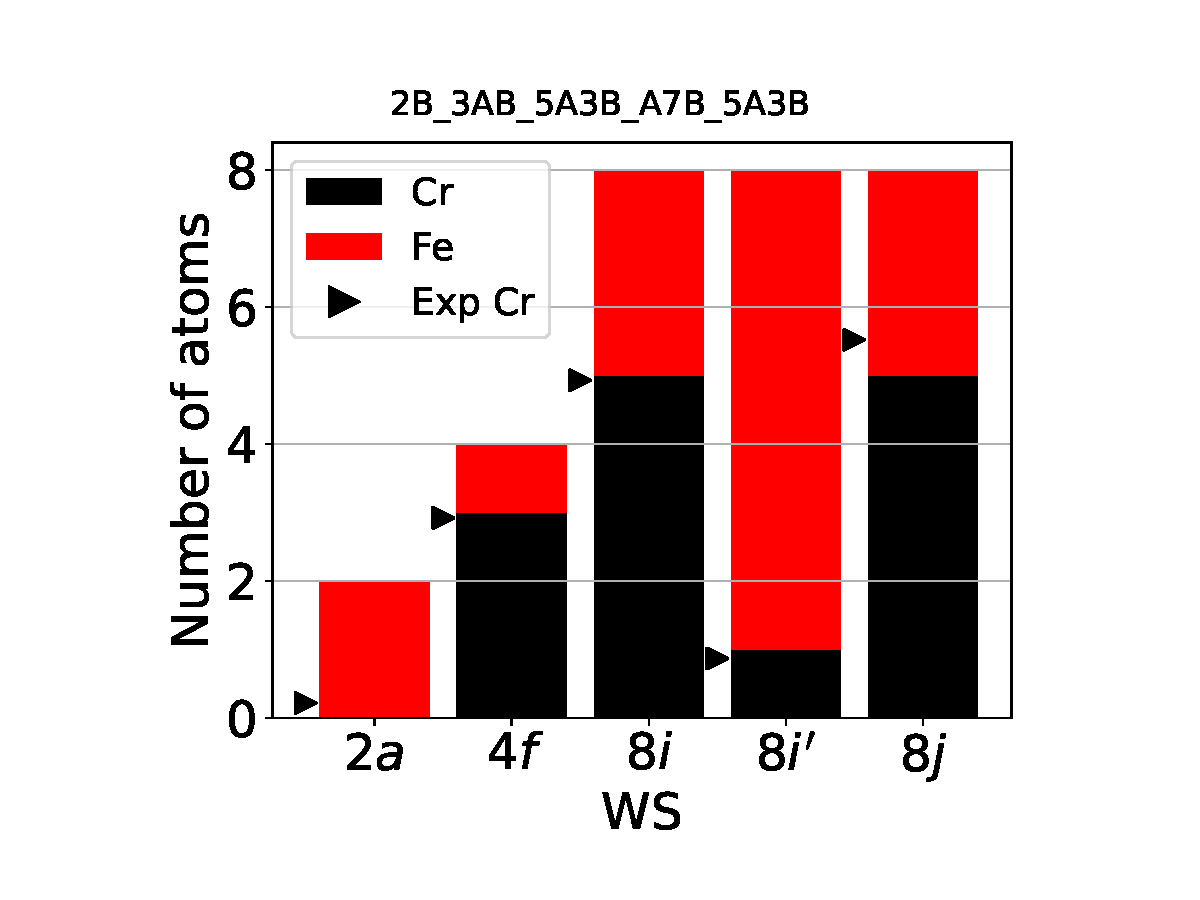
\includegraphics[height=4cm]{Figure_bdpartial_distributions.pdf}}
%  \subcaptionbox{\protect\label{fig:PartialOccupanciesB}}{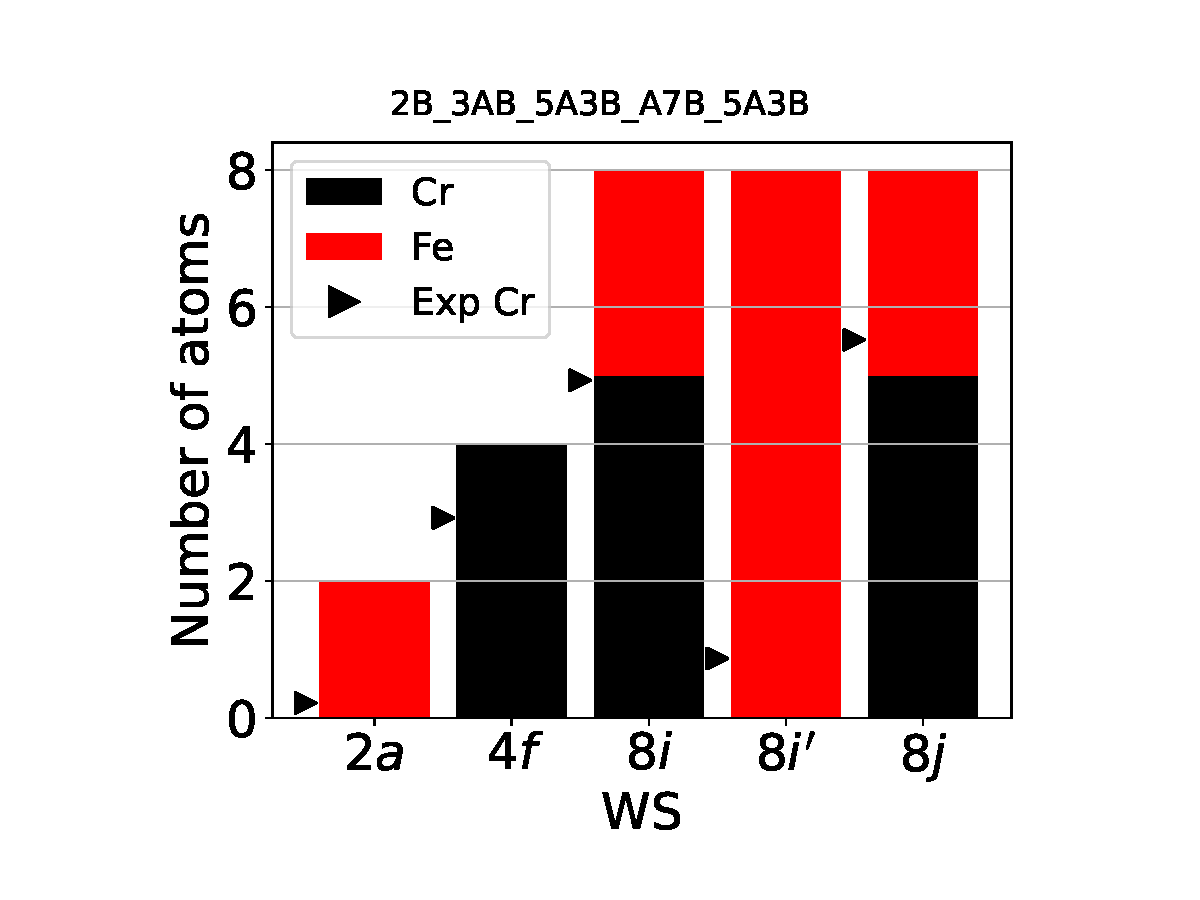
\includegraphics[height=4cm]{Figure_bdfull_distributions.pdf}}
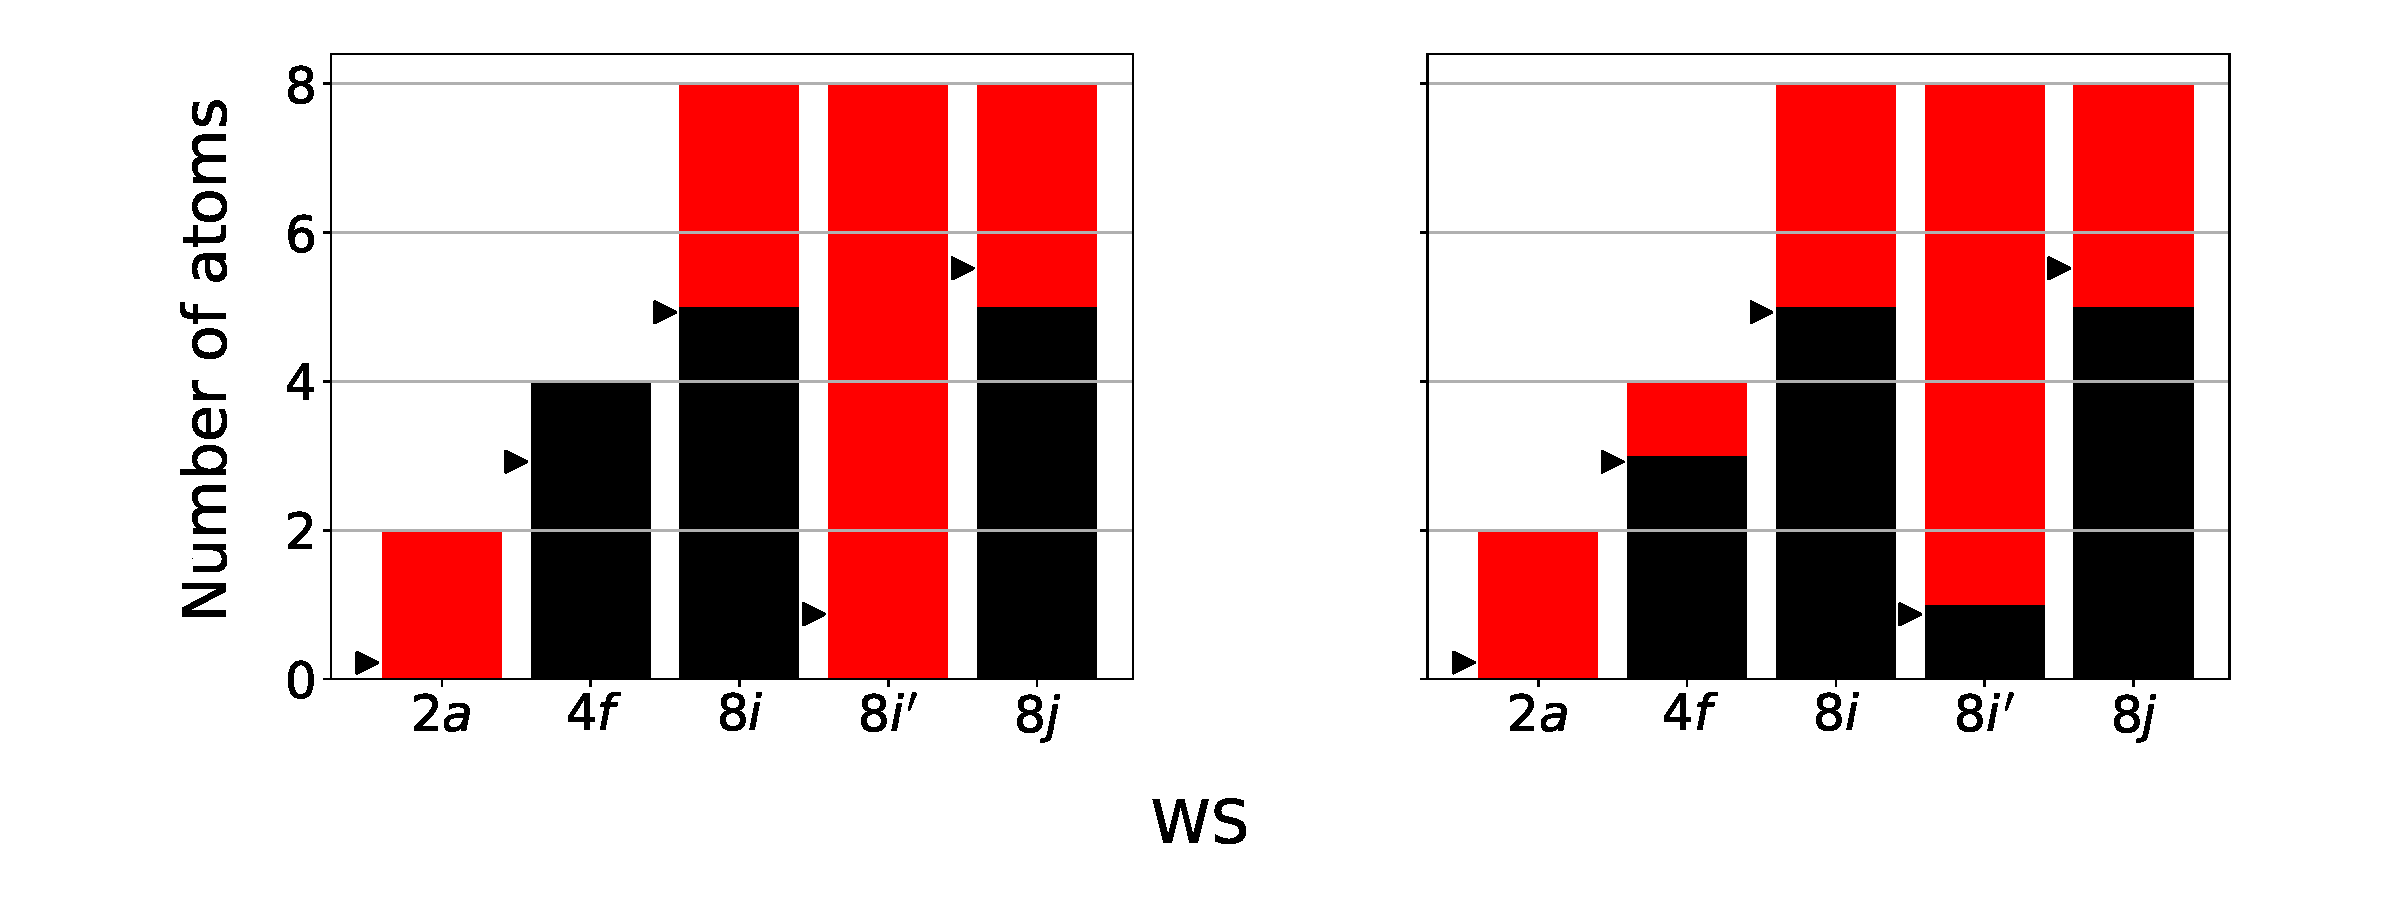
\includegraphics[height=4cm]{Figure_both_distributions.pdf}
  \caption{\protect\label{fig:PartialOccupancies}
    First model of unit cell with partial occupancy, right panel shows model B2\_A3B\_A5B3\_AB7\_A5B3 and left pannel 
    shows the further simplified model B2\_A3B2\_A5B3\_8B\_A5B3.
    \MFnew{
    \begin{itemize}
        \item Add same plot but for FO in same nominal composition
        \item add labels for Fe/Cr (maybe in white over the bars)
        \item write Whyckoff sites
        \item add titles (FO, PO1, PO2, FO-Fe\textsubscript{16}Cr\textsubscript{14})
    \end{itemize}
    
    }
  }
\end{figure}

\section{Results}

In a full sublattice model, the Fe-Cr~\textsigma~phase exhibits a tetragonal unit cell in the space group P4\textsubscript{2}/mnm in the entire composition range.  
Our results show that partial occupancy disrupts unit cell symmetry, significantly affecting the mechanical response of the \textsigma-phase.  
Using \textit{spglib*}~\cite{Spglib_Togo} as implemented in the \textit{atomistic simulation environment}~\cite{HjorthLarsen_2017}, we find that even before full optimization of the unit cell, the only decoration of the lattice  sites according to the partial occupancy breaks the tetragonal symmetry of the sigma phase.  
\MFmarginpar{*}{}{would it be possible that occupancy in 2a recovers symmetry somehow?}
Upon decoration, all the configurations acquire a triclinic unit cell with space group P1. 
The cell vector lengths and angles of the optimized triclinic cells are shown in \autoref{fig:SymmetryConsiderations} for all the configurations.  
Although small, the introduced structural variations might affect the mechanical properties of the \textsigma phase. 

\begin{figure}[H]
  \subcaptionbox{\protect\label{subfig:angle_symmetry_rupture}}{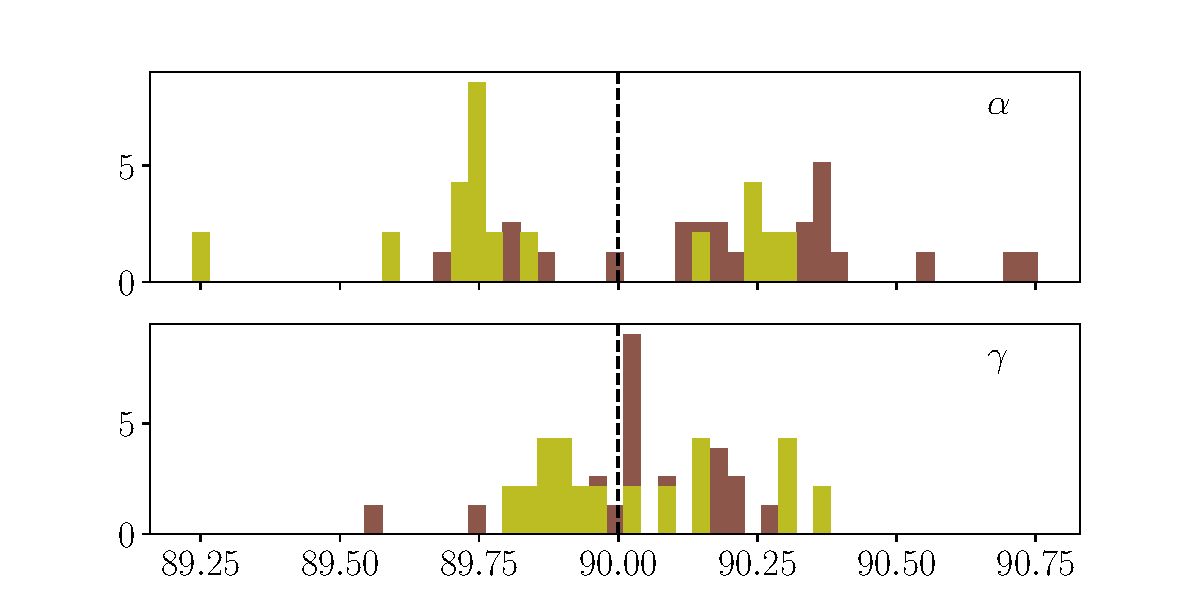
\includegraphics[height=4cm, trim=1.5cm 0cm 1.5cm 1cm, clip]{Figure_alfa_gamma_plots.pdf}}
  \subcaptionbox{\protect\label{subfig:FormationEnergies}}{\includegraphics[height=5cm, trim=0cm 0.9cm 0cm 1cm]{Figure_ConvexHull0K.pdf}}
  \caption{
    \protect\label{fig:SymmetryConsiderations}
    Effect of partial offupancy on unit cell geometry and stability. 
    (\autoref{subfig:angle_symmetry_rupture}) Distribution of $\alpha$ and $\gamma$ angles for models with partial occupancy after full optimization with DFT. 
    (\autoref{subfig:FormationEnergies}) Formation enthalpy at 0K for the full occupancy model and the two models with partial occupancy.
    }
\end{figure}

\paragraph{phase stability}

The calculated convex hull for the full occupancy samples and both models with partial occupancy is shown in \autoref{subfig:FormationEnergies}. 
The formation enthalpies of the \textsigma~phase are possitive for all compositions, which indicate that it it could be stabilized by entropy contributions. 
In the other hand, at the composition of interest, introducing partial occupancy stabilizes the phase as several samples have a formation enthalpy below the tie-line of the full-occupancy convex hull. 
In contrast, the samples at the same composition but with full occupancy lay several tens of meV/at avobe the convex hull tie line.
No direct correlation between the formation enthalpy and unit cell distoritions is observed within the chosen samples.

\paragraph{Elastic constants}

The elastic tensor of a tetragonal unit cell can be reduced to 6 independent components.
In Voigt notation~\cite{golesorkhtabar_elastic_2013}:

\begin{equation}
  \begin{pmatrix}
    C_{11} & C_{12} & C_{13} & 0 & 0 & 0 \\
    C_{12} & C_{11} & C_{13} & 0 & 0 & 0 \\
    C_{13} & C_{13} & C_{33} & 0 & 0 & 0 \\
    0 & 0 & 0 & C_{44} & 0 & 0 \\
    0 & 0 & 0 & 0 & C_{44} & 0 \\
    0 & 0 & 0 & 0 & 0 & C_{66} \\
  \end{pmatrix}
\end{equation}

In the other hand, the triclinic unit cell has 21 independent components where none of them is necesarily zero. 
In consequence, the same amount of parametrized deformations should be applied.
In addition, for each deformation tensor enough parameters should be applied as to determine each of the elastic tensor components after a least squares fit.
This makes the determination of the elastic tensor of the non-symmetrical triclinic unit cell unfeasible in the whole configurational space.

 However, we calculated an ad-hoc selection of 25 configurations for each model. 
 In \autoref{fig:OccupancyEffect} we report the changes in the VRH averaged elastic moduli with nominal composition and fractional occupation of the sublattices and its relation to formation energy.
 First, the results for the FO samples clealy show the stiffening of the compound with increasing stability (lower frmation enthalpy at 0K).
 We also see that the PO samples follow the same trend.
 A slight stiffening of the compound is already displayed for the small DFT dataset.

\begin{figure}[H]
  \fbox{ 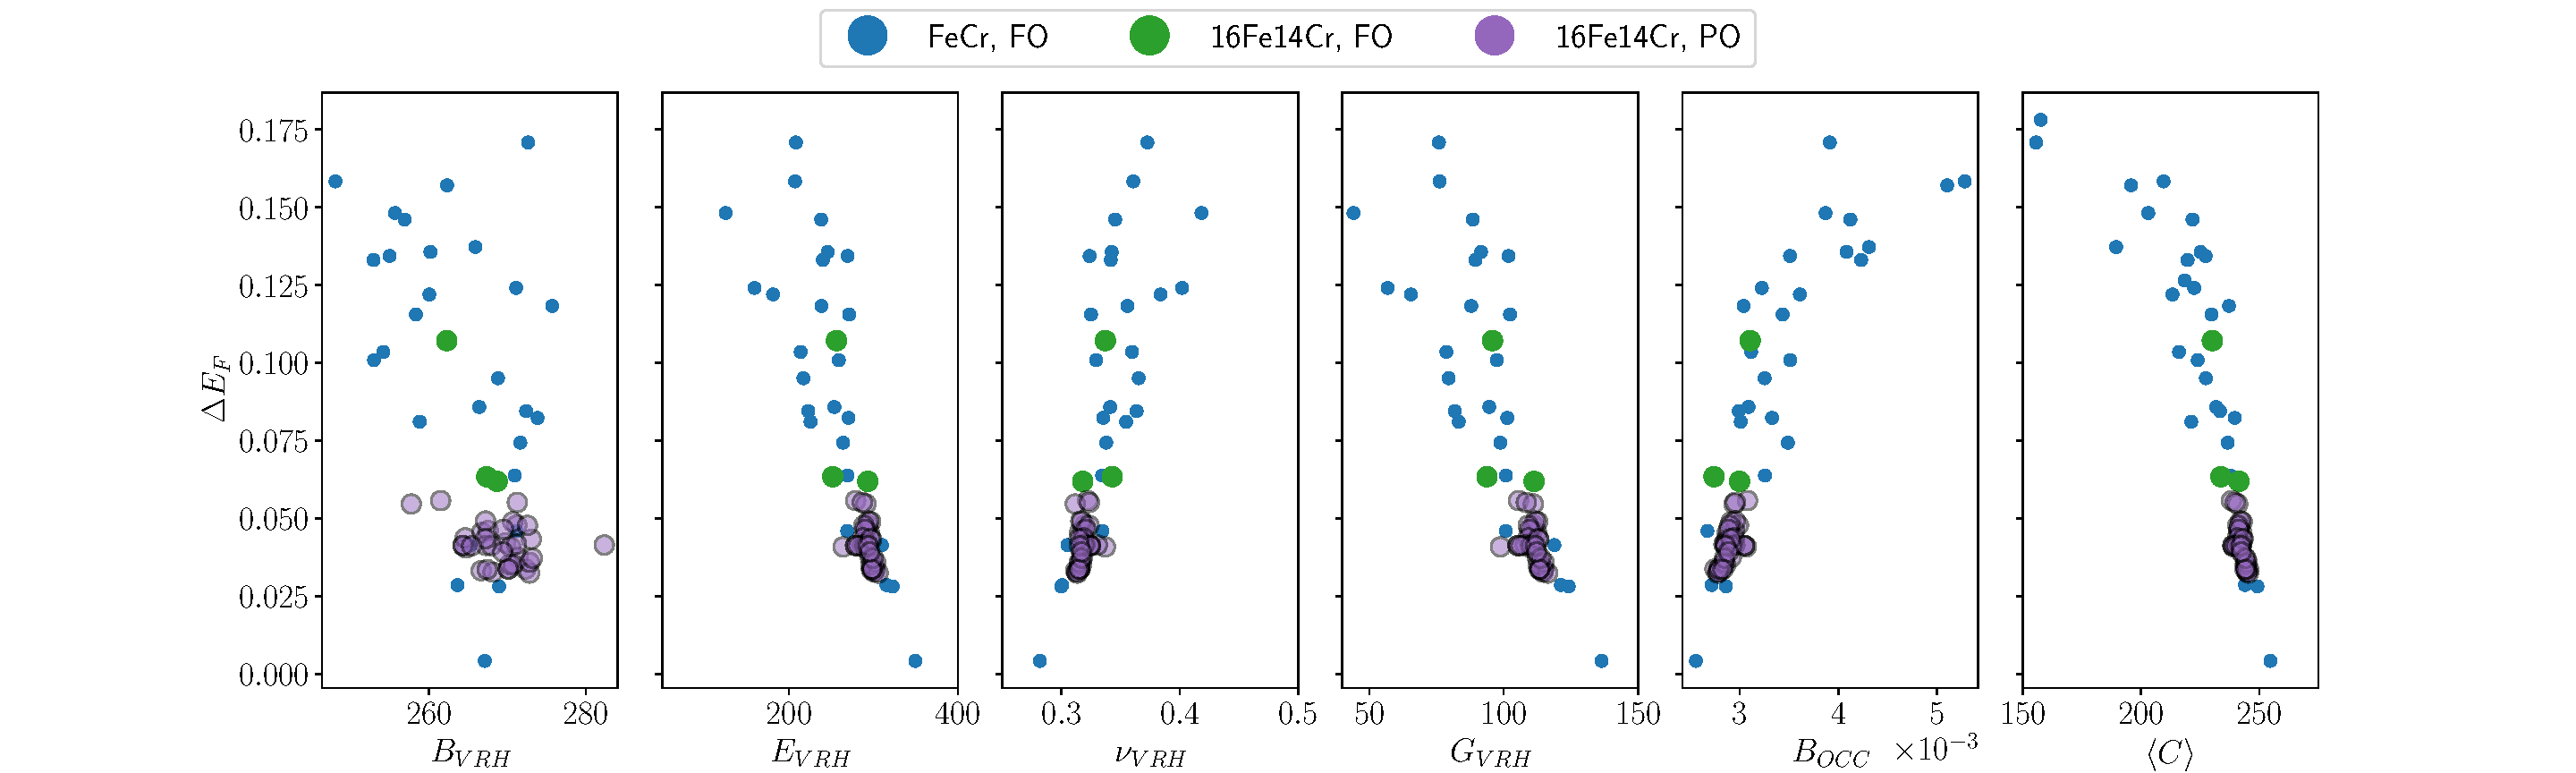
\includegraphics[width=\textwidth, trim=3.5cm 0cm 4cm 0cm, clip]{Figure_AverageElasticConstants.pdf}}
 \caption{\protect\label{fig:OccupancyEffect}
  Effect of occupancy on the stability and properties of the Fe\textsubscript{16}Cr\textsubscript{14} \textsigma ~phase.
 }
\end{figure}


 \begin{figure}[H]
  \subcaptionbox{\protect\label{fig:ElasticTensorRatios}}{{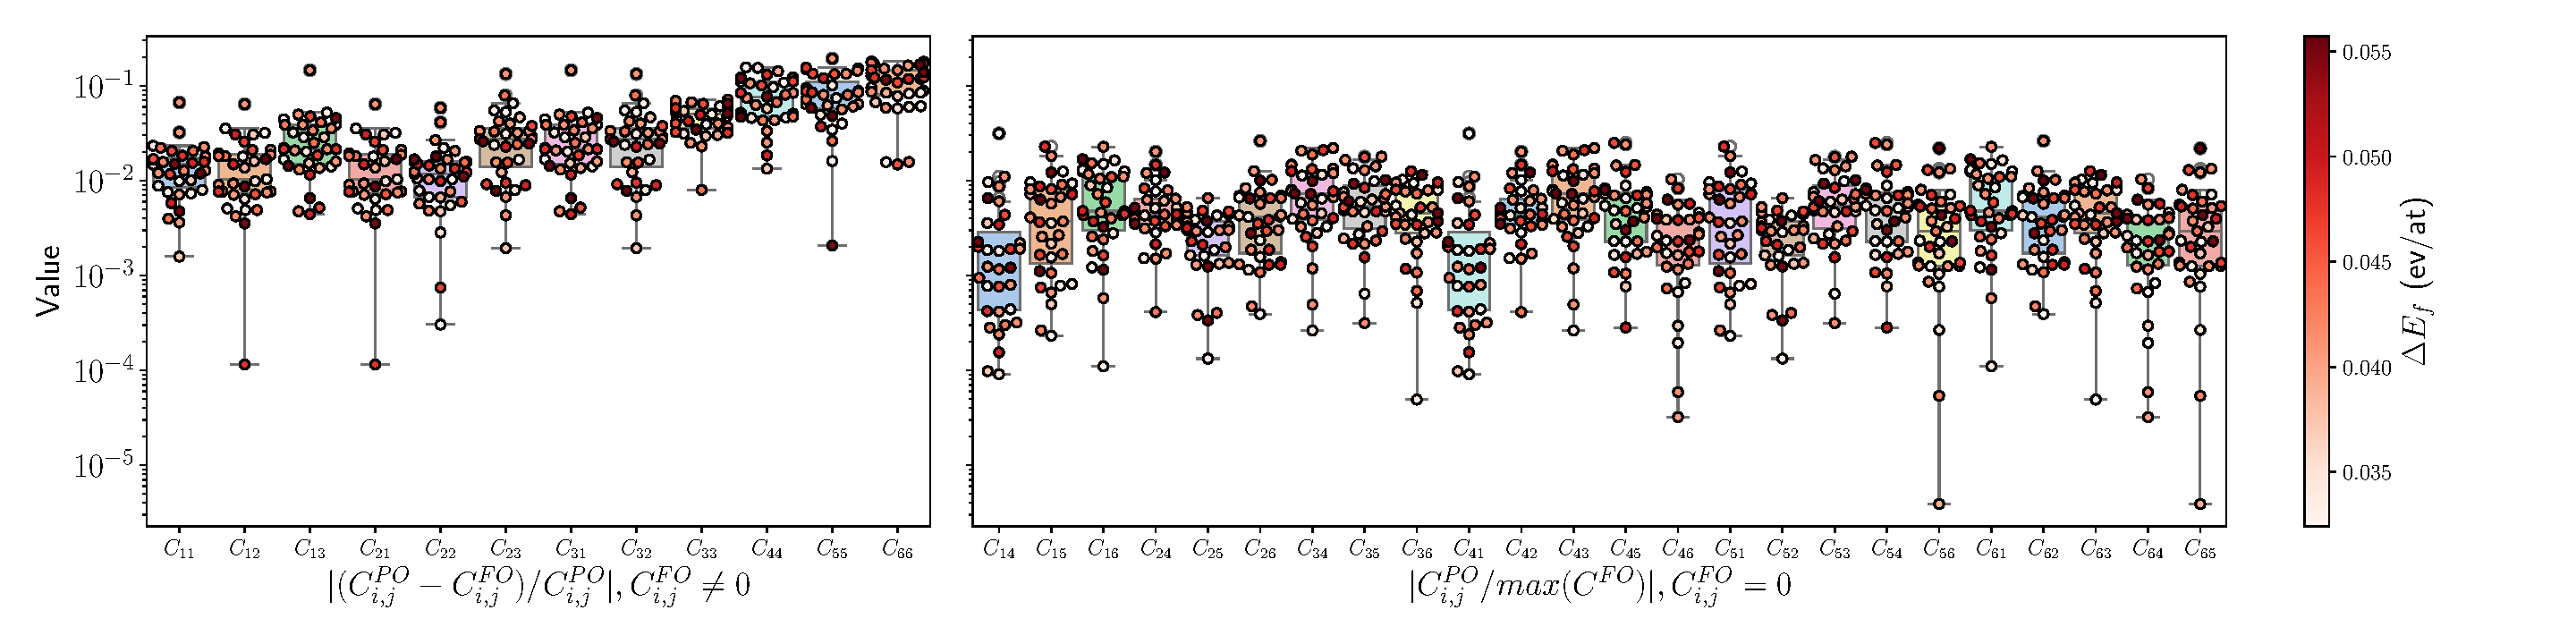
\includegraphics[width=0.6\linewidth, trim=1.2cm 0cm 6cm 0cm, clip]{Figure_swarm_allrelations.pdf}}}
  \subcaptionbox{\protect\label{fig:ElasticTensorMains}}{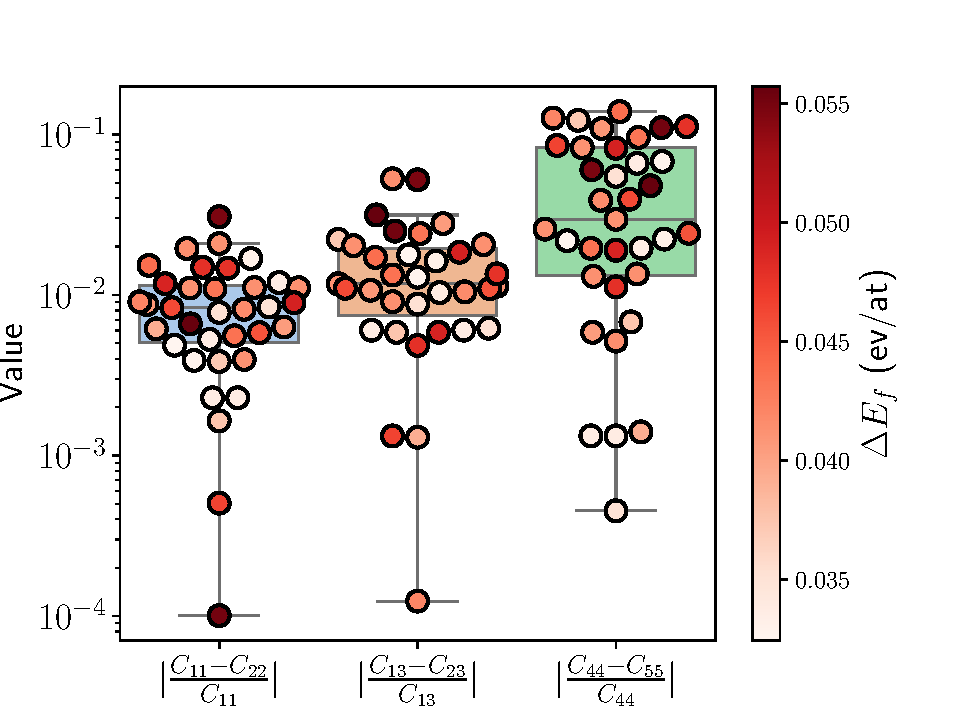
\includegraphics[width=0.3\linewidth, trim=0.5cm 0cm 1.7cm 1cm, clip]{Figure_C11_C13_C44_Deviations_on_equals.pdf}}
  \caption{\protect\label{fig:ResultsElasticConstants} 
    Comparison between elastic tensor components of the tetragonal, full occupancy (FO) model and the triclinic,
    partial occupancy (PO) model. 
    Formation energy of the samples is indicated in color code in units of eV/atom.
    (\subref{fig:ElasticTensorMains}) relative differences in the triclinic model for components that are equal in the tetragonal model. 
    (\subref{fig:ElasticTensorRatios}) relative change of the elastic tensor component between the PO samples and FO samples, for non-zero valued constants in the triclinic cell (left). 
    For the constants that zero in the tetragonal cell, we present the relative change with respect to the largest constant of the tetragonal cell (right).
  }
\end{figure}

\subsection{Machine learning extension of the sample space}

So far, we gained an approximated idea of the effect of partial occupancy on the elastic constants of the Cr--Fe \textsigma ~ phase.
However, the configuration space is only partially explored, and the 50 samples chosen for explicit elastic constant calculations is probably far from being statistically significant for the around 100k samples of the full configurational space. 

At the same time, the already performed calculations can give us valuable information about the compound after symmetry has been broken by partial occupancy. 
Valuable information about force-stress-displacement relationships can be extracted from the already performed DFT calculations which can be used to train a machine learning interatomic potential (MLIP) with a high degree of specificity. 
In this direction, we extend our dft dataset by including not only optimization and elastic constnats calculations already analyzed, but also nearest neighbour (NN) expansions of the bcc, fcc, and hcp unary unit cells of the constitutents (Fe and Cr) and random deformations including isotropic compresion and expansions and atom-position shaking.
The calculaton cost of this extension is much lower than the explicit calculation of elastic constants for probably hundreds of samples in the combinatorial exploration.
The resulting energy - NN relationship is shown in \autoref{fig:DFTDataset}.
We perform a ACE\MFnew{[ref ACE]} potential fitting using python-ace\MFnew{[ref pace]} package.
The distributions of the target variables (energies, forces, stresses) are shown in the supplementary material, as well as the fitting detapace.

The final potential can approximate our DFT formation energies with a relatively low error, as shown in \MFnew{Figure}.

\begin{figure}[H]
  \includegraphics[width=\textwidth]{Figure_DFTDataset.pdf}
  \caption{\protect\label{fig:DFTDataset}
		DFT dataset used to train the MLIP.
		The dataset includes unary unit cells, random deformations, and elastic constant calculations.
		The energy - NN relationship is shown in the right panel.
	}

\end{figure}

\begin{figure}
  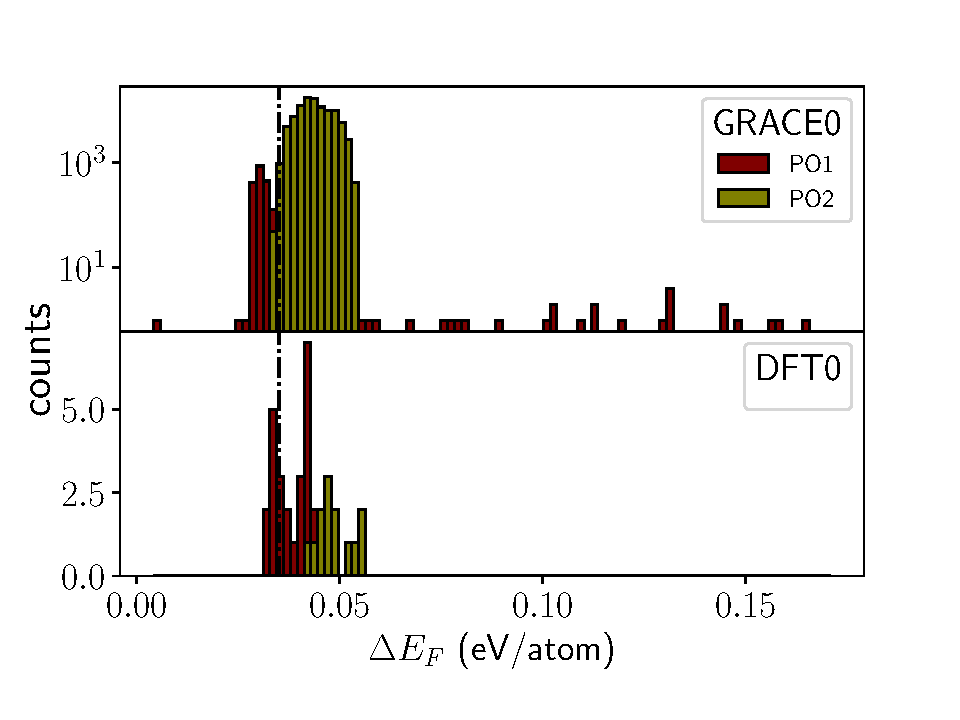
\includegraphics[width=0.6\textwidth]{Figure_GRACE_potential_prediction.pdf}
  \includegraphics[width=0.3\textwidth]{example-image-a}

  \caption{\protect\label{fig:MLIPPrediction}
    (a) Comparison between DFT and MLIP formation energies for the Fe-Cr \textsigma~phase. 
    The upper pannel shows the distribution of the DFT formation energies on the PO samples from DFT calculatiosn (blue) and the GRACE potential (purple). 
    For the latter, the full configuration space was calculated.
   In the lower panel, the parity plot between the FO, PO, and validation sets is shown. An RMSE = \MFnew{show rmse} is obtained for the predictions. 
   (b) Elastic constants for the validation set. 
	}

\end{figure}

\section{Conclusion}

In this work, we are presenting a methodical study of the effects of partial occupancy in the properties of the \textsigma phase of the FeCr system.
For the first time, the properties of this phase are calculated taking into account the experimentally observed partial occupancies.
We demonstrate that partial occupancy significantly influences the mechanical response of the \textsigma-phase, which cannot be captured by the traditional full sublattice models.
Our results provide new insights into the mechanical behavior of the Fe-Cr \textsigma-phase and highlight the importance of considering partial occupancy in theoretical models.

\section{selection of working alloy}
final long term goal is CrMnFeCoNi (order by atomic number).
We select the easiest binary with $\sigma$ phase.
We select 16Fe14Fe because it was close to the experimental 50\%Fe and it is easy to distribute between the sublattices.
show experimental partial occupancies, and the modelled distributions.
(there are slides)
explaining breaking of symmetry by partial occupancies with figures.

\section*{Acknowledgements} 

This work is a part of the project ”Artificial Intelligence for Intermetallic Materials”–AIIM funded by the Deutsche Forschungsgemeinschaft (DFG No. 505643559). 
\bibliographystyle{naturemag} \bibliography{main.bib}

\end{document}
